\section{Evaluation}
\label{sec:evaluation}

\subsection{Experimental Setup}

We evaluate eight conditions of reviewer context against three puzzles from the Age of Empires corpus. Table~3 summarizes the eight conditions, which vary along a single axis: what information is present in the reviewer context beyond the puzzle text and scoring rubric. The conditions are not nested in a strict sense---C4 (philosophy only) and C5 (lens only) decompose C6 (full profile) rather than extending it---but together they form a factorial exploration of which profile components drive evaluation quality.

\begin{table}[h]
\centering
\caption{Eight conditions in the profile ablation. Each condition specifies what reviewer context is present; the puzzle text and six-dimension scoring rubric are identical across all conditions.}
\begin{tabular}{llp{6cm}}
\toprule
Condition & Label & Context present \\
\midrule
C0 & Bare baseline & Nothing (role label only) \\
C1 & Rubric only & Six-dimension rubric with dimension definitions \\
C2 & Principles compact & Design principle names and representative quotes \\
C3 & Principles full & Names, quotes, and operational test descriptions \\
C4 & Philosophy only & Reviewer design worldview; no structured lens \\
C5 & Lens only & Structured review checklist; no biography or philosophy \\
C6 & Full profile & Complete v2 profile (current system) \\
C7 & Profile + Principles & Full profile plus all design principles (C6 + C3) \\
\bottomrule
\end{tabular}
\label{tab:conditions}
\end{table}

The three puzzles under evaluation are drawn from the Age of Empires hunt (``Wololo''). \textbf{Puzzle I} (Dark Age round) is a civilization-identification extraction puzzle in which solvers identify Age of Empires II civilizations from clued characteristics and extract a letter from each; the intended answer is CASTLE. \textbf{Puzzle II} (Feudal Age round) is a bracket tournament puzzle in which known and unknown historical figures compete according to domain-specific criteria, with the winner determined by game-mechanic rules; the intended answer is ONAGER. \textbf{Puzzle III} (Castle Age round) is a technology chain completion puzzle in which solvers reconstruct a research dependency graph and extract from the terminal nodes; the intended answer is LOOM. All three puzzles were developed independently of the reviewer profiles; no profile content refers to these specific puzzles.

The same three reviewers---Dan Katz, Thomas Snyder, and Dana Young---appear in all eight conditions, ensuring that reviewer selection does not introduce between-condition variance. Scores are reported on the 30-point scale (six dimensions, 1--5 each) with a pass threshold of 22/30. Where a single reviewer number is reported, it represents the panel's composite score. Full per-reviewer breakdowns are available in the supplementary data.

\subsection{Score Results}

Table~4 reports scores for all eight conditions across the three puzzles, alongside the number of named analytical frameworks introduced and the count of actionable fix suggestions. Figure~\ref{fig:ablation} presents the same data as a grouped bar chart with the pass threshold marked.

% Figure 2: Ablation bar chart — 8 conditions × 3 puzzles
%
% DEPENDENCIES: main.tex must include:
%   \usepackage{tikz}
%   \usepackage{pgfplots}
%   \usepgflibrary{patterns}
%   \pgfplotsset{compat=1.18}
%
% Colors by condition type:
%   C0  light gray    (bare baseline)
%   C1  medium gray   (rubric only)
%   C2  light blue    (principles compact)
%   C3  medium blue   (principles full)
%   C4  green         (philosophy only)
%   C5  orange        (lens only)
%   C6  dark blue     (full profile — current system)
%   C7  dark gray     (profile + principles)

\begin{figure}[t]
\centering
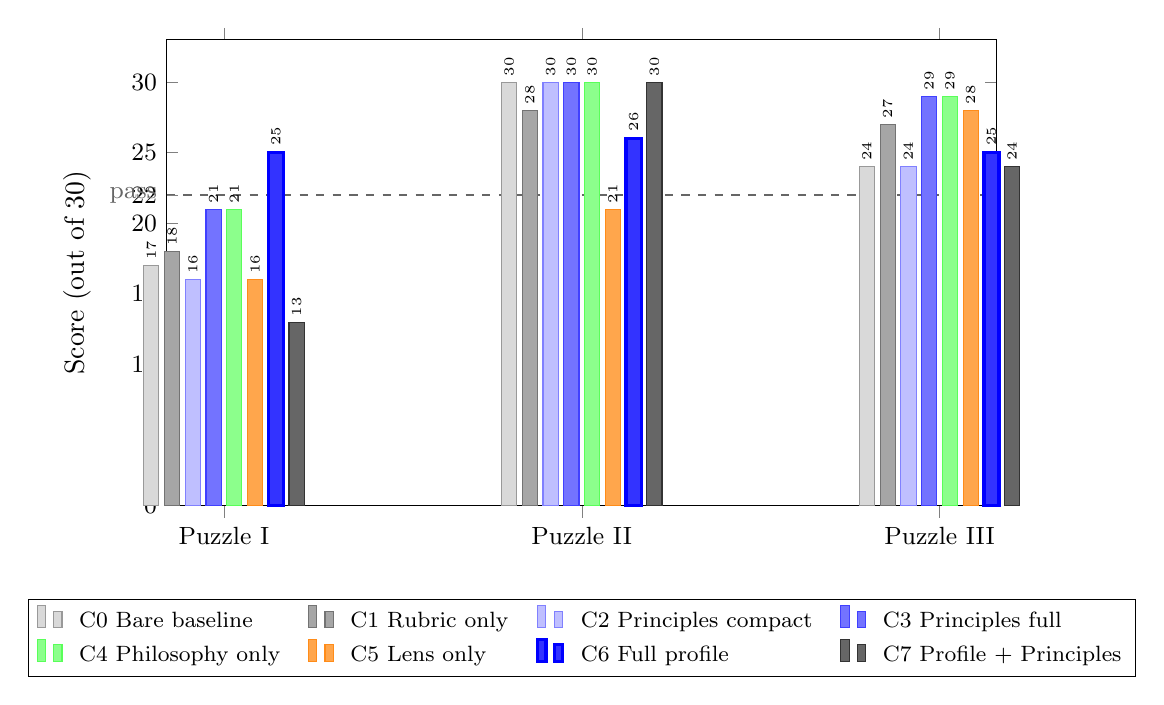
\begin{tikzpicture}
\begin{axis}[
    ybar,
    bar width=5.5pt,
    width=\textwidth,
    height=7.5cm,
    enlarge x limits=0.08,
    ylabel={Score (out of 30)},
    ymin=0,
    ymax=33,
    ytick={0,5,10,15,20,22,25,30},
    yticklabel style={font=\small},
    extra y ticks={22},
    extra y tick style={
        grid=major,
        grid style={dashed, thick, black!60},
        tick label style={font=\small\itshape, color=black!60}
    },
    extra y tick labels={pass},
    symbolic x coords={Puzzle I, Puzzle II, Puzzle III},
    xtick=data,
    xticklabel style={font=\small},
    legend style={
        at={(0.5,-0.20)},
        anchor=north,
        legend columns=4,
        font=\footnotesize,
        column sep=4pt,
        /tikz/every even column/.append style={column sep=8pt},
    },
    legend cell align=left,
    nodes near coords,
    nodes near coords style={font=\tiny, rotate=90, anchor=west, inner sep=2pt},
    nodes near coords align={vertical},
    every node near coord/.append style={/pgf/number format/.cd, fixed, precision=0},
    grid=none,
    axis on top=false,
    clip=false,
]

% C0 — Bare baseline — light gray
\addplot[fill=black!15, draw=black!40] coordinates {
    (Puzzle I,  17)
    (Puzzle II, 30)
    (Puzzle III,24)
};

% C1 — Rubric only — medium gray
\addplot[fill=black!35, draw=black!55] coordinates {
    (Puzzle I,  18)
    (Puzzle II, 28)
    (Puzzle III,27)
};

% C2 — Principles compact — light blue
\addplot[fill=blue!25, draw=blue!50] coordinates {
    (Puzzle I,  16)
    (Puzzle II, 30)
    (Puzzle III,24)
};

% C3 — Principles full — medium blue
\addplot[fill=blue!55, draw=blue!75] coordinates {
    (Puzzle I,  21)
    (Puzzle II, 30)
    (Puzzle III,29)
};

% C4 — Philosophy only — green
\addplot[fill=green!45, draw=green!65] coordinates {
    (Puzzle I,  21)
    (Puzzle II, 30)
    (Puzzle III,29)
};

% C5 — Lens only — orange
\addplot[fill=orange!70, draw=orange!90] coordinates {
    (Puzzle I,  16)
    (Puzzle II, 21)
    (Puzzle III,28)
};

% C6 — Full profile (current system) — dark blue, prominent
\addplot[fill=blue!80, draw=blue!100, line width=1.2pt] coordinates {
    (Puzzle I,  25)
    (Puzzle II, 26)
    (Puzzle III,25)
};

% C7 — Profile + Principles — dark gray
\addplot[fill=black!60, draw=black!80] coordinates {
    (Puzzle I,  13)
    (Puzzle II, 30)
    (Puzzle III,24)
};

\legend{
    C0 Bare baseline,
    C1 Rubric only,
    C2 Principles compact,
    C3 Principles full,
    C4 Philosophy only,
    C5 Lens only,
    C6 Full profile,
    C7 Profile + Principles
}

\end{axis}
\end{tikzpicture}

% Annotation strip below the chart
\vspace{4pt}
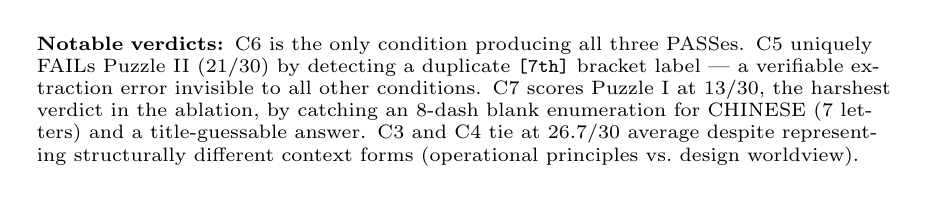
\begin{tikzpicture}[font=\scriptsize]
\node[anchor=west, text width=0.9\textwidth, align=left] at (0,0) {%
    \textbf{Notable verdicts:}
    C6 is the only condition producing all three PASSes.
    C5 uniquely FAILs Puzzle~II (21/30) by detecting a duplicate \texttt{[7th]} bracket label --- a verifiable extraction error invisible to all other conditions.
    C7 scores Puzzle~I at 13/30, the harshest verdict in the ablation, by catching an 8-dash blank enumeration for CHINESE (7 letters) and a title-guessable answer.
    C3 and C4 tie at 26.7/30 average despite representing structurally different context forms (operational principles vs.\ design worldview).%
};
\end{tikzpicture}

\caption{Score by condition and puzzle across the 8-condition ablation. All conditions produce 0 named frameworks in C0--C1; C2 introduces principle-name vocabulary; C3--C7 produce domain-specific analytical frameworks. The pass threshold (22/30, dashed) shows that only C6 (full profile) produces consistent passes across all three puzzles. C5 uniquely detects a verifiable defect in Puzzle~II; C7 scores Puzzle~I harshest by catching a factual error.}
\label{fig:ablation}
\end{figure}


\begin{table}[h]
\centering
\caption{Ablation results. Scores are out of 30; pass threshold is 22. PASS/FAIL designations appear in parentheses. ``Frameworks'' counts named evaluative concepts introduced in the review text. ``Fixes'' counts actionable revision suggestions, with qualitative characterizations noted.}
\begin{tabular}{llrrrrrrl}
\toprule
Cond. & Label & P-I & P-II & P-III & Avg & Frameworks & Fixes \\
\midrule
C0 & Bare baseline     & 17 (F) & 30 (P) & 24 (P) & 23.7 & 0  & $\sim$2 (generic) \\
C1 & Rubric only       & 18 (F) & 28 (P) & 27 (P) & 24.3 & 0  & 4 (structural) \\
C2 & Principles compact & 16 (F) & 30 (P) & 24 (P) & 23.3 & 10 & 6 (named) \\
C3 & Principles full   & 21 (F) & 30 (P) & 29 (P) & 26.7 & 11 & 5 (2 critical) \\
C4 & Philosophy only   & 21 (F) & 30 (P) & 29 (P) & 26.7 & 9  & 5 (2 critical) \\
C5 & Lens only         & 16 (F) & 21 (F) & 28 (P) & 21.7 & $\sim$8 & 8 (most defects) \\
C6 & Full profile      & 24.7 (P) & 26.3 (P) & 25.0 (P) & 25.3 & 6 & 5 (actionable) \\
C7 & Profile + Princ.  & 13 (F) & 30 (P) & 24 (P) & 22.3 & 14 & 7 (harshest) \\
\bottomrule
\end{tabular}
\label{tab:ablation}
\end{table}

The most salient observation is that the score gradient across conditions is \emph{not monotonic}. If profile depth were the primary driver of score, the gradient C0 $\to$ C1 $\to$ C2 $\to \cdots \to$ C7 would produce increasing scores. It does not. C2 (principles compact, 10 named frameworks, average 23.3) scores \emph{lower} than C1 (rubric only, 0 named frameworks, average 24.3). Providing principle names and associated quotes---without operational tests specifying how to apply them---makes assessment vocabularily richer but evaluatively less calibrated: the reviewer applies named criteria as filters without the grounding machinery needed to distinguish a real failure from a borderline case.

C3 and C4, by contrast, both reach an average of 26.7/30 despite representing structurally different forms of reviewer context (C3 provides operational tests; C4 provides design worldview without a structured lens). We interpret this as evidence that evaluative signal can be encoded in multiple representational forms: a reviewer who reasons from a coherent design philosophy navigates borderline cases differently from a reviewer who applies a checklist, but the aggregate accuracy of their verdicts is comparable when both forms of context are complete.

The most practically important pattern in the score table involves the per-puzzle verdict profile rather than the per-condition average. C6 (full profile, the current system) is the \emph{only} condition that produces passing scores on all three puzzles. Every other condition either fails a puzzle it should pass (C5 fails Puzzle II; C7 fails Puzzle I) or fails a puzzle it might be reasonable to fail (C0 through C4 all fail Puzzle I, which may contain genuine defects---see Section~\ref{sec:defects} below). The interpretation of this observation requires some care, because the ``correct'' verdict for Puzzle I is itself contested; we return to this in the defect detection discussion.

The harshest single-puzzle score in the entire ablation is C7's 13/30 on Puzzle I, lower by a substantial margin than any other condition's score on any puzzle. Adding design principles to a complete profile does not consistently improve calibration---it produces a more demanding reviewer whose additional sensitivity occasionally finds real problems (the blank-count error described below) but whose aggregate verdict on Puzzle I falls well below what any other condition produces.

\subsection{Framework Emergence}
\label{sec:frameworks}

The qualitative signal in the framework count column is at least as informative as the score column. C0 and C1 produce zero named evaluative frameworks across all three puzzles: the reviewer may identify that a puzzle has a clarity problem or an elegance problem, but the critique is cast entirely in the rubric's own vocabulary, producing statements like ``the extraction mechanism is not clearly communicated'' without a named concept that transfers to other puzzles or other design contexts.

C2 introduces ten named frameworks---but they are \emph{injected} principle names, the same names that appear in the context provided. The reviewer applies vocabulary from the input rather than generating vocabulary from evaluative experience. The frameworks named are, in that sense, retrieved rather than emergent: they are the principle names, applied as criteria, with quotes as supporting evidence. This is not without value, but it is a different phenomenon from what C6 produces.

C6 (full profile, current system) names six frameworks across the three puzzle reviews. None of these six frameworks appears in any input provided to the reviewer. The frameworks surfaced are: \emph{a-ha economy} (Foggy Brume), characterizing whether the puzzle's aha moment is expended efficiently or squandered through redundancy; \emph{load-bearing test} (Thomas Snyder), the operation of removing individual constraints to verify that each element forces something in the solution; \emph{world-model consistency} (Emily Short), whether the puzzle's logic is coherent within the fictional or factual universe it invokes; \emph{social fabric} (Jordan Weisman), whether the puzzle's design accommodates team-solving dynamics or implicitly assumes solitary reconstruction; \emph{perceptual-shift} (Scott Kim), whether the solver experiences a genuine reframing of the problem or merely accumulates information until an answer becomes apparent; and \emph{visual grammar} (Dana Young), whether the diagrammatic elements of a puzzle communicate structure through their arrangement rather than through labels alone.

These frameworks did not exist in any input text. They are the reviewer's evaluative vocabulary---surfaced by the profile's encoded design philosophy and characteristic concerns, and applied to the specific features of each puzzle under review. This is the primary qualitative distinction between C2 and C6: both name frameworks, but C2 names principle-labels and C6 names domain-emergent analytical tools that a practitioner might adopt and apply to their own future work.

C7's count of 14 frameworks reflects the union of profile frameworks and principle-names. The blend is not strictly additive: some principle-names appear alongside profile frameworks that cover the same ground, producing reviews that are terminologically dense without proportional gain in evaluative precision. The redundancy analysis in Section~\ref{sec:redundancy} characterizes this more precisely.

\subsection{Defect Detection}
\label{sec:defects}

The most striking finding in the ablation is not a score comparison but a binary defect-detection result. C5 (lens only---the structured review checklist without biography or design philosophy) gave Puzzle II a score of 21/30, uniquely falling below the pass threshold on a puzzle that six other conditions passed. The reason is traceable to a specific, verifiable error in the puzzle's ASCII bracket diagram.

In Puzzle II, the bracket tournament is represented as a text-art diagram with positions labeled by round and seed: \texttt{[QF-1]}, \texttt{[QF-2]}, \texttt{[SF-1]}, \texttt{[SF-2]}, and so on. The diagram as constructed contains a duplicate label: the position that should read \texttt{[SF-1][5th]} instead reads \texttt{[SF-1][7th]}, reusing the \texttt{[7th]} label that also appears at \texttt{[QF-2]}. A solver navigating the diagram by seed extraction rather than by inference from surrounding context will extract \texttt{S} from the incorrectly labeled position rather than \texttt{E}, producing a wrong answer without receiving any signal that an error has occurred. This is not a quality judgment---it is a binary correctness failure: one solver path through the puzzle is broken.

No condition other than C5 identified this error. The lens checklist's specificity about visual design communicating structure---``does the diagram's visual arrangement make the extraction path unambiguous, or does it require inference to compensate for layout failures?''---made the duplicate label visible in a way that neither scoring criteria nor design philosophy nor operational principles did. The biography-free, philosophy-free character of C5 appears to have concentrated its attention specifically on the visual-mechanical properties of the puzzle artifact rather than on higher-level evaluative concerns.

A parallel observation applies to Puzzle I in C7. The combination of Verify the Last Mile (from the principles context) with the profile's structural analysis surfaced an error in the puzzle's answer enumeration: Bonus clue C is presented with eight answer blanks (\texttt{\_ \_ \_ \_ \_ \_ \_ \_}), but the intended answer, CHINESE, has seven letters. This is a factual error in the puzzle's construction, not a difficulty or elegance judgment. C7 also noted that CASTLE is partially guessable from the puzzle's title before completing the extraction, which the Surprise the Answer principle flags as a confirmation failure. C6 did not catch either of these issues.

The implication is that C5 and C7 function as \emph{defect-detection instruments} while C6 functions as a \emph{calibrated quality evaluator}. For practitioners, this suggests a two-pass evaluation protocol: run C6 first for overall quality calibration and actionable feedback, then run C5 as a verification pass specifically looking for mechanical and visual failures that higher-level evaluation frameworks may not surface. The three non-redundant principles from C7 (discussed in Section~\ref{sec:redundancy}) could be added to C5 to construct a compact defect-detection condition without the full overhead of C7.

\subsection{Redundancy Analysis}
\label{sec:redundancy}

C7 reviews included explicit meta-commentary from reviewers about which principles added information beyond what their profile already covered. This commentary, though not systematically prompted, allows us to characterize which principle injections produce unique evaluative signal and which are subsumed by well-designed profiles.

Three principles were consistently identified as adding signal not already present in the reviewer profile:

\textbf{Verify the Last Mile} was the only context element that prompted reviewers to trace the extraction mechanism character by character, checking that each step from raw answer material to final answer word is unambiguous and executable. No profile lens item performs this operation at this granularity; the principle is apparently specific enough to activate a mode of review that profile-level framing does not.

\textbf{Blame the Player} introduced a retrospective solver affect dimension---how a solver feels at the moment of discovering that an error or ambiguity was the puzzle's fault rather than their own. Profile lenses are generally designer-centric (what choices did the constructor make?) rather than solver-retrospective (what does the solver experience when the puzzle fails?). This principle consistently introduced a perspective that profiles did not.

\textbf{Snyder's Computer Test} was noted as adding unique signal despite the fact that the Thomas Snyder profile extensively documents the philosophy behind the test. The principle, when injected explicitly, prompts the reviewer to \emph{apply} the test rather than merely reason in its spirit. The profile encodes the worldview; the explicit principle triggers the operation.

Three principles were consistently identified as redundant with full profiles:

\textbf{Solving = Proving Understanding} was characterized as subsumed by each profile's engagement lens, which asks whether the puzzle verifies that the solver has understood the domain rather than merely guessing or brute-forcing. The principle captures the same requirement in a more abstract formulation, but the profile lens already operationalizes it.

\textbf{No Over-Scaffolding} was subsumed by profile lens items that ask explicitly whether the puzzle provides more structure than the solving process requires---a check that appears in multiple profile lenses under domain-specific formulations (``Does the extraction mechanism telegraph the answer before the domain knowledge is applied?'').

\textbf{The Riven Standard} was subsumed by profile items addressing theme-structure alignment: whether the puzzle's content domain is load-bearing in the mechanism or merely decorative. Multiple profiles include a variant of this check under the reviewer's characteristic domain concerns.

The practical recommendation from this analysis is that practitioners using complete domain-specific profiles should supplement with exactly the three non-redundant principles and omit the rest. The total context overhead is modest (three principle descriptions add approximately 400 tokens to a full-profile context), and the gain in defect coverage is, per the C7 data, real and traceable to specific verifiable errors.
